\documentclass[main.tex]{subfiles}
 
\begin{document}
In this final chapter, we 

\section{SciGRID data}
The SciGRID dataset needs to be translated into the our model, as it contains more information than we need, not yet in the desired format. 

\subsection{Properties}
\emph{(A more detailed analysis of dataset properties is available on the GitHub repository.)}

Before any processing, we find that the SciGRID network (obtained from \texttt{PyPSA} example code, the exact dataset used by \cite{Nesti2018emergentfailures}) contains 585 buses, 1423 generators (of all sources) and 489 loads. It also contains 38 storage units (all are pumped hydroelectric), but these were excluded from our analysis.\footnote{More specifically, they were used in solving the OPF problem, but their initial charge was set to zero.} There are 852 transmission lines in the dataset, at possible voltage levels $220 \, \si{\kilo\volt}$ and $380 \, \si{\kilo\volt}$, and there are 96 transformers (between these two voltages). Transmission lines have per-kilometre estimates for admittance, from which the total admittance can be deduced.

\subsubsection{Voltages}
In our model, we \emph{normalise} the grid voltage. To do so, we multiply all line admittances by the \emph{square} of their operating voltages, after which all voltages can be assumed to be $1$, and a unit of current is proportional to a unit of transmitted power. Of the 585 buses, 192 are part of one of the 96 \emph{voltage pairs}: these are two buses at the same location, with the same name (except for the voltage suffix), connected via a transformer. By merging these pairs, we find 489 geographically unique buses, at normalised voltage. From now on, we will refer to these (possibly merged) buses as the buses of the network: $n=489$, $\mathcal{N} = \range{489}$.

\subsubsection{Loads}
There is exactly 1 load connected to each bus. In reality, there are of course thousands of loads connected to a bus, but the load in the dataset is the \emph{aggregated} load at that bus. We have hourly time series (\ie amount of $\si{\mega\watt}$ being consumed) for each node in the year 2011, which only includes active power consumption.

\subsubsection{Generators}
Generators are connected to the geographically closest bus, and there is at most one generator per bus of each type.\footnote{In order of installed capacity: \emph{Wind Onshore} ($37\,\si{\giga\watt}$), \emph{Solar} ($37\,\si{\giga\watt}$), \emph{Hard Coal} ($25\,\si{\giga\watt}$), \emph{Gas} ($24\,\si{\giga\watt}$), \emph{Brown Coal} ($21\,\si{\giga\watt}$), \emph{Nuclear} ($12\,\si{\giga\watt}$), \emph{Run of River} ($4\,\si{\giga\watt}$), \emph{Other} ($3\,\si{\giga\watt}$), \emph{Wind Offshore} ($3\,\si{\giga\watt}$), \emph{Oil} ($2.7\,\si{\giga\watt}$), \emph{Waste} ($1.6\,\si{\giga\watt}$), \emph{Storage Hydro} ($1.4\,\si{\giga\watt}$), \emph{Multiple} ($0.15\,\si{\giga\watt}$) and \emph{Geothermal} ($32\,\si{\mega\watt}$).} This means that generation is \emph{aggregated}: multiple generators of the same type are combined into one. There are 489 solar generators, 488 onshore wind generators and 5 offshore wind generators. Offshore wind generators are connected to buses at the north coast of Germany. This means that every bus houses stochastic generation. Their geographic distribution is shown in Figure~\ref{fig:solarwind}.

\subsubsection{Lines}
Line voltages and admittances are normalised as described above. For each line, we have the names of the two original buses that it connects, which can easily be converted to the new bus collection.

During the study of cascading failures, we found that the network contains \emph{parallel lines}: lines that connect the same pairs of buses. In some cases, there are up to four different lines that are all parallel. When examining these cases on OpenStreetMap, we find that there are indeed parallel lines in the physical network. This is reflected by the \emph{lengths} of parallel lines, as given by SciGRID: these are not the great-circle distances between buses, but rather the distance measured along the line (which makes some turns and bends).

Because our model only holds for \emph{digraphs}, which cannot have parallel lines, we \emph{combine} parallel lines, by summing their (voltage normalised) admittances, and summing their thresholds.\footnote{The results regarding the kernel of $\FRT$, and the Optimised method for analysis cascading failures, break down without this property.} \cite{Nesti2018emergentfailures} do not mention this anomaly, and use the original set of lines. For comparison, we computed some results for both versions of the network, and found the results to be somewhat similar, in general. Because we did not consider the case of parallel lines in our model, combining parallel lines in the dataset seems like the \emph{correct} choice.

Of the 852 original lines, there are 705 unique links between original buses before normalising voltages, and there are 695 unique links between buses. There are never two parallel lines with opposite orientation. These 695 lines were used in our model, and will be referred to as simply the \emph{lines} of the network: $m = 695$.

\section{Bus covariance}


\section{Line covariance}

By incorporating bus covariances in our model (which result from correlated weather), we hope to find new structure in the line covariances. 
To assess the effect of estimating bus covariances, we compare three possible bus covariance matrices:
\begin{enumerate}
	\item \emph{The identity matrix}: all bus injections are independently Gaussian distributed with the same variance. (They are almost IID, but their means differ.)
	\item \emph{The diagonal of estimated variances}: all bus injections are independently Gaussian distributed, but their variances and means differ.
	\item \emph{The estimated covariances}: the vector of bus injections is (multivariate) Gaussian distributed. All bus injections are, in general, dependent on each other, and their variances and means differ.
\end{enumerate}

We expect the covariance of a random pair of lines to be relatively low, when their physical separation (measured either in kilometres or in graph distance) is high. 
Because weather is correlated, even at high distance, using the bus full covariance might result in higher covariances between lines with high separation. (This was concluded by \cite{Nesti2018emergentfailures}.) 

Using a different bus covariance matrix will likely result in a overall increase or decrease of line covariances. Note, however, that the line covariance matrix is scaled by an arbitrary factor $\epsilon$, so any overall change in covariance has no significance in the model. \todo{Maar als je normaliseert op variantie?}

\towrite{Compare three bus covariance }


\begin{figure}
    \centering
    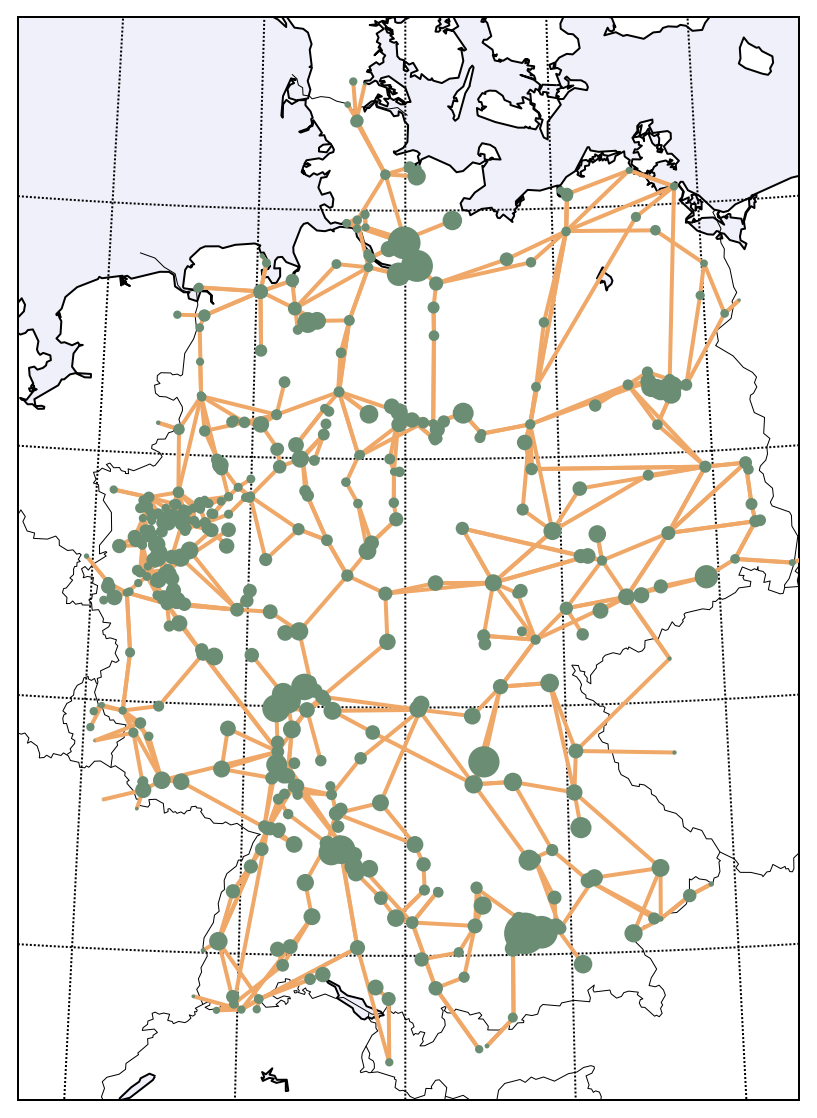
\includegraphics[width=.4\textwidth]{img/load.png}
    \caption{PLACEHOLDER: The load distribution of Germany at ???.}
    \label{fig:loaddistribution}
\end{figure}
\begin{figure}
    \centering
    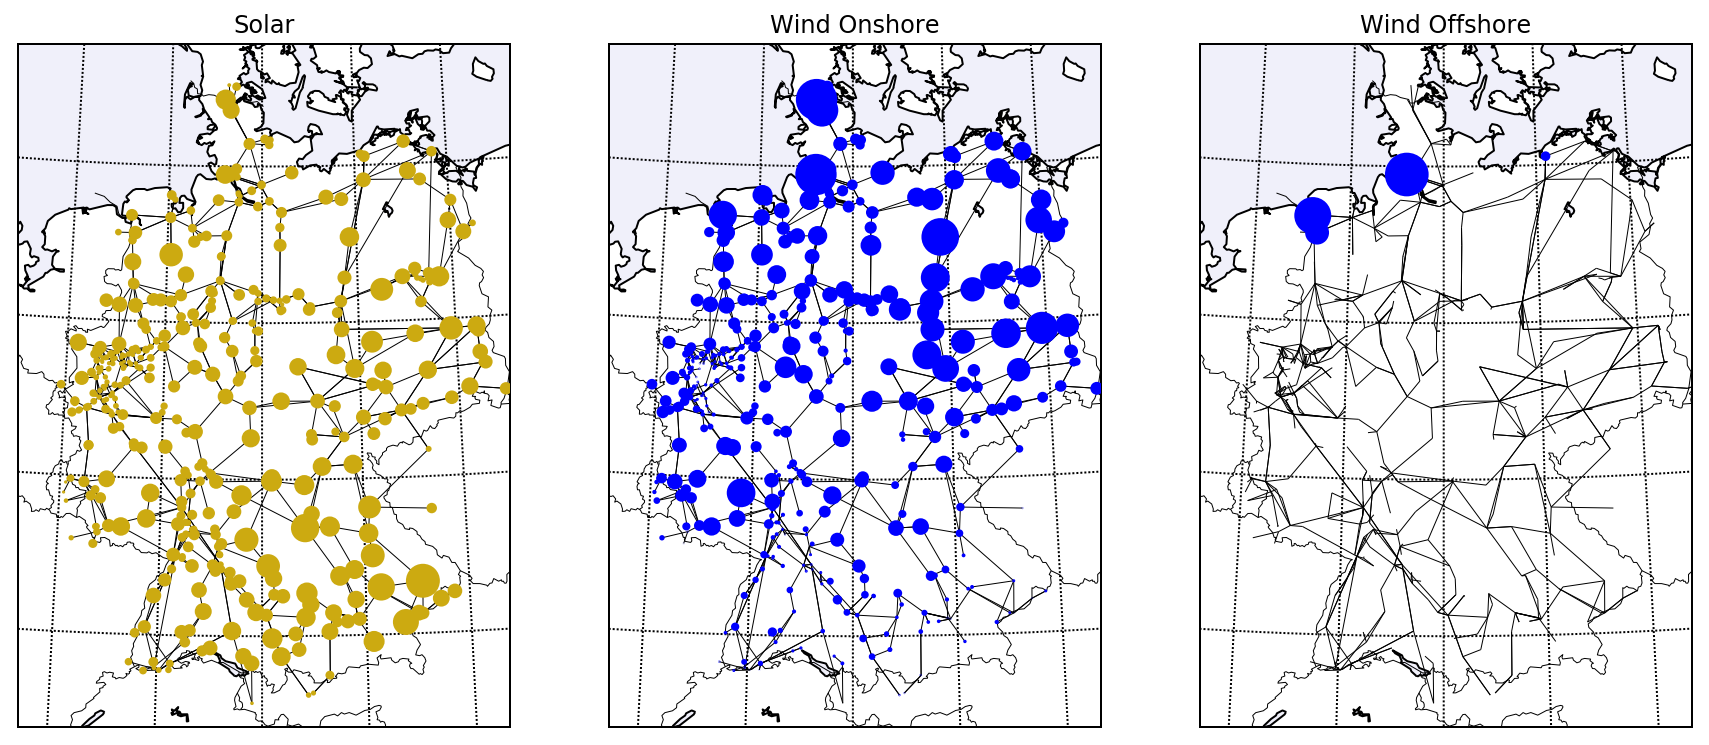
\includegraphics[width=\textwidth]{img/solarwind.png}
    \caption{PLACEHOLDER: Solar, wind onshore, wind offshore generation at ?? in Germany.}
    \label{fig:solarwind}
\end{figure}
\begin{figure}
    \centering
    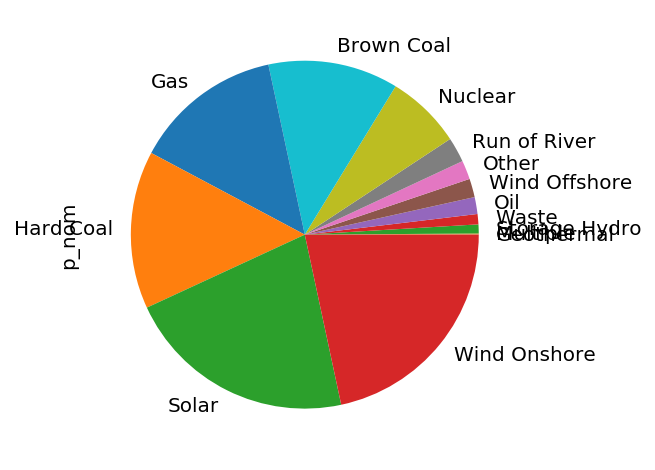
\includegraphics[width=.4\textwidth]{img/genprop.png}
    \caption{PLACEHOLDER: Generation capacity technology shares in Germany in 2011.}
    \label{fig:generationtech}
\end{figure}
\begin{figure}
    \centering
    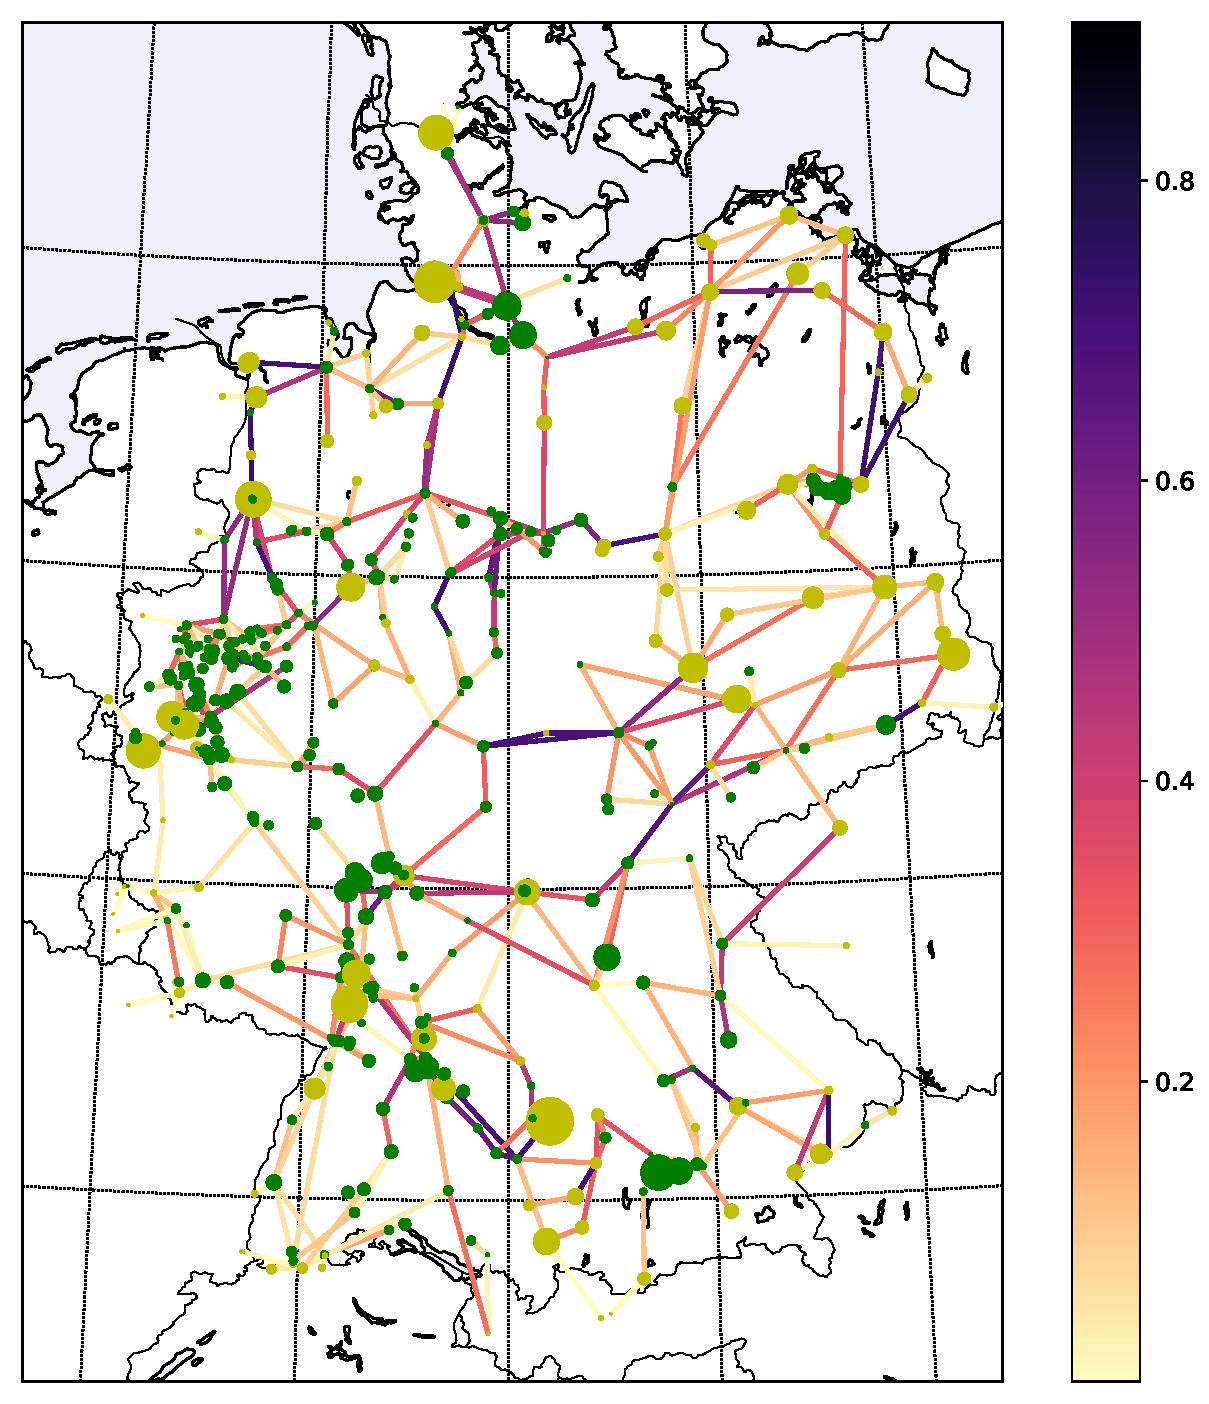
\includegraphics[width=.6\textwidth]{img/nominallineflow.pdf}
    \caption{Nominal line flow during 11:00-12:00, as fraction of line capacity. Node size represents net power injection. When generation exceeds load, the injection is positive (yellow), otherwise negative (green). \emph{Compare with Figure 1a of \cite{Nesti2018emergentfailures}.}}
    \label{fig:generationtech}
\end{figure}
asdf

\todo{Plotjes van kansen zoals in \label{stochasticpowerinjections}}

\begin{table}[]
    \centering
    \begin{tabular}{c|ccrr|ccrr}
\toprule
\multicolumn{1}{c}{} & \multicolumn{4}{c}{\textsc{Solar}} & \multicolumn{4}{c}{\textsc{Wind}} \\
\midrule
\multicolumn{1}{c}{} & 
\multicolumn{1}{c}{\textit{default}} & \multicolumn{1}{c}{\textit{modified}} & 
\multicolumn{1}{c}{1\%} & \multicolumn{1}{c}{2\%} & 
\multicolumn{1}{c}{\textit{default}} & \multicolumn{1}{c}{\textit{modified}} & 
\multicolumn{1}{c}{1\%} & \multicolumn{1}{c}{2\%} \\
\midrule
Jan & \texttt{385} & \texttt{\textbf{484}} & \texttt{\textbf{5}} & \texttt{\textbf{0}} & \texttt{\textbf{488}} & \texttt{488} & \texttt{\textbf{0}} & \texttt{\textbf{0}} \\
Feb & \texttt{364} & \texttt{\textbf{485}} & \texttt{\textbf{4}} & \texttt{\textbf{0}} & \texttt{\textbf{487}} & \texttt{487} & \texttt{\textbf{0}} & \texttt{\textbf{1}} \\
Mar & \texttt{334} & \texttt{\textbf{475}} & \texttt{\textbf{14}} & \texttt{\textbf{0}} & \texttt{\textbf{487}} & \texttt{487} & \texttt{\textbf{1}} & \texttt{\textbf{0}} \\
Apr & \texttt{211} & \texttt{\textbf{477}} & \texttt{\textbf{11}} & \texttt{\textbf{1}} & \texttt{\textbf{488}} & \texttt{488} & \texttt{\textbf{0}} & \texttt{\textbf{0}} \\
May & \texttt{189} & \texttt{\textbf{473}} & \texttt{\textbf{16}} & \texttt{\textbf{0}} & \texttt{\textbf{467}} & \texttt{467} & \texttt{\textbf{21}} & \texttt{\textbf{0}} \\
Jun & \texttt{255} & \texttt{\textbf{481}} & \texttt{\textbf{8}} & \texttt{\textbf{0}} & \texttt{\textbf{480}} & \texttt{480} & \texttt{\textbf{8}} & \texttt{\textbf{0}} \\
Jul & \texttt{292} & \texttt{\textbf{485}} & \texttt{\textbf{4}} & \texttt{\textbf{0}} & \texttt{\textbf{488}} & \texttt{488} & \texttt{\textbf{0}} & \texttt{\textbf{0}} \\
Aug & \texttt{179} & \texttt{\textbf{478}} & \texttt{\textbf{10}} & \texttt{\textbf{1}} & \texttt{\textbf{488}} & \texttt{488} & \texttt{\textbf{0}} & \texttt{\textbf{0}} \\
Sep & \texttt{259} & \texttt{\textbf{472}} & \texttt{\textbf{16}} & \texttt{\textbf{1}} & \texttt{\textbf{487}} & \texttt{487} & \texttt{\textbf{1}} & \texttt{\textbf{0}} \\
Oct & \texttt{263} & \texttt{\textbf{480}} & \texttt{\textbf{9}} & \texttt{\textbf{0}} & \texttt{\textbf{488}} & \texttt{488} & \texttt{\textbf{0}} & \texttt{\textbf{0}} \\
Nov & \texttt{290} & \texttt{\textbf{472}} & \texttt{\textbf{17}} & \texttt{\textbf{0}} & \texttt{\textbf{486}} & \texttt{486} & \texttt{\textbf{2}} & \texttt{\textbf{0}} \\
Dec & \texttt{317} & \texttt{\textbf{482}} & \texttt{\textbf{7}} & \texttt{\textbf{0}} & \texttt{\textbf{486}} & \texttt{486} & \texttt{\textbf{2}} & \texttt{\textbf{0}} \\
\bottomrule
    \end{tabular}%TODO: modified wind bold?
    \caption{Number of buses (out of 489 solar, 488 wind) for which the ARMA model could be fitted using either the \emph{default} implementation of \texttt{arima} in \texttt{R}, or the \emph{modified} version (described in \ref{arimamod}).
    \newline
    When even the modified method yielded no results, uniform noise was added to the series before fitting. Noise magnitude was set to 1\% of generation capacity, or 2\% when needed.
    \newline
    Figures in \textbf{bold} indicate which results are used.
    %All nodes now have usable results.
    }
    \label{tab:arimafitstats}
\end{table}
failures
\begin{table}
\begin{tabular}{lll}
\toprule
$l$ & $\PROB \left[ |\mel{f}_l| \geq 1 \right]$ & $\mel{I}_l$ \\
\midrule
361 & 3.45\hphantom{0}\% &  1.65 \\
516 & 2.91\hphantom{0}\% &  1.79 \\
586 & 2.75\hphantom{0}\% &  1.84 \\
587 & 2.73\hphantom{0}\% &  1.85 \\
803 & 2.02\hphantom{0}\% &  2.10 \\
670 & 1.21\hphantom{0}\% &  2.54 \\
19  & 1.13\hphantom{0}\% &  2.60 \\
302 & 1.08\hphantom{0}\% &  2.64 \\
48  & 1.03\hphantom{0}\% &  2.68 \\
554 & 0.974\% &  2.73 \\
\midrule
488 & 0.971\% &  2.73 \\
809 & 0.824\% &  2.88 \\
28  & 0.748\% &  2.96 \\
810 & 0.728\% &  2.98 \\
29  & 0.396\% &  3.53 \\
27  & 0.355\% &  3.62 \\
389 & 0.247\% &  3.95 \\
390 & 0.245\% &  3.96 \\
486 & 0.235\% &  4.00 \\
249 & 0.056\% &  5.30 \\
\bottomrule
\end{tabular}

\caption{TODO}
\label{tab:top20}
\end{table}

\section{Previous work}
This thesis was inspired by \cite{Nesti2018emergentfailures}, and we have verified their results. Our results are in overall agreement, with some minor differences. \todo{minder beknopt}

Verschillen:

- lijnen samengevoegd

- geen arma maar diff

- cascades gegeven van top 10


Kritiek op nesti:

- ARMA modellen, logisch? nodig? goede modellen?

- geeft cascades niet van top 10

- ze nemen een contingency factor van 0.7 bij de OPF (arbitrair) maar voor de analyse van cascades niet. (toch?)




\clearpage
\end{document}